% Edit this section directly. Styling is in raylo-report.sty.
\section{The machine-learning tier: the linear classifier}
The classifier that has carried the residual since August is a linear support vector machine on character-level TF-IDF features. In plain terms, it counts the character fragments that appear in the merchant string and bank narrative, and learns a straight-line boundary between each category and the rest. It is the standard first model for short, noisy text: it trains in minutes, occupies 65 megabytes, scores about a thousand rows per second on one CPU core, and anything more elaborate has to beat it. It was preferred over logistic regression because it won on every promotion metric, and its ``don't answer when unsure'' behaviour works from its own decision margin.

Since August the model itself has not changed. What changed is the data it learned from, and the current version, v8, is the reference for every comparison in section 9.

\subsection{What the September data did}
The credit tranche moved accuracy on 2,000 held-out money-in transactions from 62\% to 85\%. Accuracy on debits did not move. This was the largest single-step gain in the classifier's history and it came from data, not modelling.

For high-risk categories the honest starting point, after the leak was removed, was 48\% on the 174 risk-category rows that reach the classifier. Two steps followed, in order. Five new rules for card-issuer inflows and overdraft narratives took it to 59\% before any labelling. Then 5,000 labelled rows of the same population took the classifier itself to 76\%, above the 70\% bar we set for risk categories for the first time on an honest measurement.

\begin{figure}[H]
\centering
\ChartTitle{Figure 6. Linear classifier accuracy on the two September targets, step by step}
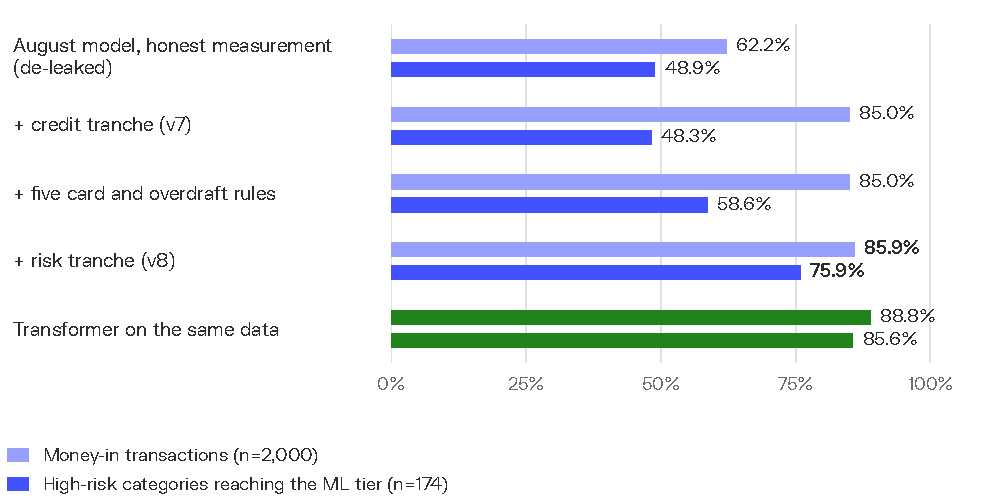
\includegraphics[width=\linewidth]{charts/fig-stair.pdf}
\caption*{The same linear model throughout; only the training data and the rules in front of it changed. The transformer row is section 9's result on identical data.}
\end{figure}
The version in the serving artefact is still v5 from August. The gap between it and v8 is now 24 points on credits and 28 points on the risk debits that reach the classifier, so promoting v8 is the zero-risk interim step whatever is decided about the transformer.

